%%%%%%%%%%%%%%%%%%%%%%%%%%%%%%%%%%%%%%%
% Wenneker Resume/CV
% LaTeX Template
% Version 1.1 (19/6/2016)
%
% This template has been downloaded from:
% http://www.LaTeXTemplates.com
%
% Original author:
% Frits Wenneker (http://www.howtotex.com) with extensive modifications by 
% Vel (vel@LaTeXTemplates.com)
%
% License:
% CC BY-NC-SA 3.0 (http://creativecommons.org/licenses/by-nc-sa/3.0/
%
%%%%%%%%%%%%%%%%%%%%%%%%%%%%%%%%%%%%%%

%----------------------------------------------------------------------------------------
%	PACKAGES AND OTHER DOCUMENT CONFIGURATIONS
%----------------------------------------------------------------------------------------

\documentclass[a4paper,12pt]{memoir} % Font and paper size

%%%%%%%%%%%%%%%%%%%%%%%%%%%%%%%%%%%%%%%%%
% Wenneker Resume/CV
% Structure Specification File
% Version 1.1 (19/6/2016)
%
% This file has been downloaded from:
% http://www.LaTeXTemplates.com
%
% Original author:
% Frits Wenneker (http://www.howtotex.com) with extensive modifications by 
% Vel (vel@latextemplates.com)
%
% License:
% CC BY-NC-SA 3.0 (http://creativecommons.org/licenses/by-nc-sa/3.0/)
%
%%%%%%%%%%%%%%%%%%%%%%%%%%%%%%%%%%%%%%%%%

%----------------------------------------------------------------------------------------
%	PACKAGES AND OTHER DOCUMENT CONFIGURATIONS
%----------------------------------------------------------------------------------------

\usepackage{XCharter} % Use the Bitstream Charter font
\usepackage[utf8]{inputenc} % Required for inputting international characters
\usepackage[T1]{fontenc} % Output font encoding for international characters

\usepackage[top=1cm,left=1cm,right=1cm,bottom=1cm]{geometry} % Modify margins

\usepackage{graphicx} % Required for figures

\usepackage{flowfram} % Required for the multi-column layout

\usepackage{url} % URLs

\usepackage[usenames,dvipsnames]{xcolor} % Required for custom colours

\usepackage{tikz} % Required for the horizontal rule

\usepackage{enumitem} % Required for modifying lists
\setlist{noitemsep,nolistsep} % Remove spacing within and around lists

\setlength{\columnsep}{\baselineskip} % Set the spacing between columns

% Define the left frame (sidebar)
\newflowframe{0.2\textwidth}{\textheight}{0pt}{0pt}[left]
\newlength{\LeftMainSep}
\setlength{\LeftMainSep}{0.2\textwidth}
\addtolength{\LeftMainSep}{1\columnsep}
 
% Small static frame for the vertical line
\newstaticframe{1.5pt}{\textheight}{\LeftMainSep}{0pt}
 
% Content of the static frame with the vertical line
\begin{staticcontents}{1}
\hfill
\tikz{\draw[loosely dotted,color=RoyalBlue,line width=1.5pt,yshift=0](0,0) -- (0,\textheight);}
\hfill\mbox{}
\end{staticcontents}
 
% Define the right frame (main body)
\addtolength{\LeftMainSep}{1.5pt}
\addtolength{\LeftMainSep}{1\columnsep}
\newflowframe{0.7\textwidth}{\textheight}{\LeftMainSep}{0pt}[main01]

\pagestyle{empty} % Disable all page numbering

\setlength{\parindent}{0pt} % Stop paragraph indentation

%----------------------------------------------------------------------------------------
%	NEW COMMANDS
%----------------------------------------------------------------------------------------

\newcommand{\userinformation}[1]{\renewcommand{\userinformation}{#1}} % Define a new command for the CV user's information that goes into the left column

\newcommand{\cvheading}[1]{{\Huge\bfseries\color{RoyalBlue} #1} \par\vspace{.6\baselineskip}} % New command for the CV heading
\newcommand{\cvsubheading}[1]{{\Large\bfseries #1} \bigbreak} % New command for the CV subheading

\newcommand{\Sep}{\vspace{1em}} % New command for the spacing between headings
\newcommand{\SmallSep}{\vspace{0.5em}} % New command for the spacing within headings

\newcommand{\aboutme}[2]{ % New command for the about me section
\textbf{\color{RoyalBlue} #1}~~#2\par\Sep
}
	
\newcommand{\CVSection}[1]{ % New command for the headings within sections
{\Large\textbf{#1}}\par
\SmallSep % Used for spacing
}

\newcommand{\CVItem}[2]{ % New command for the item descriptions
\textbf{\color{RoyalBlue} #1}\par
#2
\SmallSep % Used for spacing
}

\newcommand{\bluebullet}{\textcolor{RoyalBlue}{$\circ$}~~} % New command for the blue bullets
 % Include the file specifying document layout and packages

%----------------------------------------------------------------------------------------
%	NAME AND CONTACT INFORMATION 
%----------------------------------------------------------------------------------------

\userinformation{ % Set the content that goes into the sidebar of each page
\begin{flushright}
% Comment out this figure block if you don't want a photo
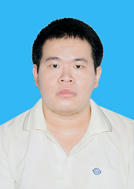
\includegraphics[width=0.6\columnwidth]{DSC_3894.jpg}\\[\baselineskip] % Your photo
\small % Smaller font size
Ho Quang Nam \\ % Your name
\url{hoquangnam45}\\
\url{@gmail.com} \\ % Your email address
+84 0978 142 040\\ % Your phone number
\Sep % Some whitespace
\textbf{Address} \\
2/4/51/14 \\ % Address 1
Le Thuc Hoach St,\\ % Address 2
Phu Tho Hoa Ward,\\ % Address 3
Tan Phu District,\\
HCM City\\ % Whitespace under this block to push it up under the photo
\end{flushright}
}

%----------------------------------------------------------------------------------------

\begin{document}

\userinformation % Print your information in the left column

\framebreak % End of the first column

%----------------------------------------------------------------------------------------
%	HEADING
%----------------------------------------------------------------------------------------

\cvheading{Ho Quang Nam} % Large heading - your name

\cvsubheading{Curriculum Vitae} % Subheading - your occupation/specialization

\CVSection{Objective}

%------------------------------------------------

%To broaden my knowledge on the field of AI and machine learning, so that i can using those knowledge to help integrate deep learning with IoT devices to help create smart devices and network with self-learning capability which can be used to help and assist people in various day-to-day tasks 
To broaden my knowledge on the field of software development and mobile development, so that i can using those knowledge to help create useful product which can be used to help and assist people in various day-to-day tasks 
%-----------------------------------------------------
%----------------------------------------------------------------------------------------
%	EDUCATION
%----------------------------------------------------------------------------------------
\Sep

\CVSection{Education}

%------------------------------------------------

\CVItem{2015 - present, HCM University of Techonology}{Candidate for Bachelor in Computer Engineering(CE)}

\CVItem{GPA: 7.29 - Toeic: 860}

%------------------------------------------------

\Sep % Extra whitespace after the end of a major section

%----------------------------------------------------------------------------------------
%	EXPERIENCE
%----------------------------------------------------------------------------------------

\CVSection{Past Experiences}

%------------------------------------------------
\bluebullet Made a chess clock on DE2i-150 FPGA Board using Verilog HDL

\bluebullet Implement a MIPS Processor using Verilog on FPGA Board that included basic addition, substraction, ...

\bluebullet Build a weather and temperature monitoring system and upload those data to Google Sheet, can also receiving remote control command over SMS and Internet

\bluebullet Write a basic Java app that capable of receive remote sensor reading and graph it

\bluebullet Use Keras framework and Python to implement a traffic sign classifier on my Internship

\bluebullet Write a basic comic website using HTML + PHP + Javascript + CSS as an assignment for my class

\bluebullet Write a basic Android app for interacting with my IoT system
%------------------------------------------------

\Sep % Extra whitespace after the end of a major section

%----------------------------------------------------------------------------------------
%	COMMUNICATION SKILLS
%----------------------------------------------------------------------------------------
%-----------------------------------------------
%----------------------------------------------------------------------------------------
%	SKILLS
%----------------------------------------------------------------------------------------

\CVSection{Skills}

%------------------------------------------------

\CVItem{Programming}
{\begin{tabular}{p{0.2\textwidth} p{0.2\textwidth} p{0.2\textwidth}}
\bluebullet Java &  \bluebullet C & \bluebullet Python\\
\bluebullet C++ &  \bluebullet HTML & \bluebullet Javascript\\
\end{tabular}}

%------------------------------------------------

\CVItem{Languages}
{\begin{tabular}{p{0.5\textwidth}}
 \bluebullet Vietnamese (Mother Tongue)\\
 \bluebullet English (Intermediate Competency - TOEIC 860)\\
\end{tabular}}

\CVItem{Knowledge}
{\begin{tabular}{p{0.5\textwidth}}
		\bluebullet Computer Architecture\\
		\bluebullet Computer Network\\
\end{tabular}}

%------------------------------------------------

\Sep % Extra whitespace after the end of a major section

%----------------------------------------------------------------------------------------
%	NEW PAGE DELIMITER
%	Place this block wherever you would like the content of your CV to go onto the next page
%---------------------------------------------------------------------------------------

%----------------------------------------------------------------------------------------
%	AWARDS
%----------------------------------------------------------------------------------------

\CVSection{Social Works}

%------------------------------------------------

\bluebullet Volunteer work at charitable restaurant

\bluebullet Blood donating

\bluebullet Helping hospital organize a New Moon Festival for unfortunate kids

\bluebullet Cleaning up streets in HCM City

%------------------------------------------------

\Sep % Extra whitespace after the end of a major section

%----------------------------------------------------------------------------------------
%	INTERESTS
%----------------------------------------------------------------------------------------

\CVSection{Personal Hobbies}

Listen to Music, Playing Games, Browsing the Web, Reading comic

%------------------------------------------------

\Sep % Extra whitespace after the end of a major section

%----------------------------------------------------------------------------------------

\end{document}
